\documentclass[11pt]{article}
\usepackage[margin=1in]{geometry}
\usepackage{amsmath,amssymb,amsthm,mathtools}
\usepackage{graphicx}
\usepackage{enumitem}
\usepackage[hidelinks]{hyperref}

\newtheorem{theorem}{Theorem}
\newtheorem{lemma}[theorem]{Lemma}
\newtheorem{remark}[theorem]{Remark}
\newcommand{\R}{\mathbb R}
\newcommand{\avgint}{\mathop{\rlap{\raisebox{.12ex}{--}}\!\int}}
\newcommand{\diam}{\operatorname{diam}}

\title{Exponent Upgrade for All \(p\)-Admissible Measures\\
\large A candidate full resolution of Remark 8.2 in arXiv:2505.20555}
\author{Autonomous proof candidate for human review}
\date{11 August 2026}

\begin{document}
\maketitle

\begin{center}
\fbox{\parbox{0.91\textwidth}{\textbf{Status.}
Candidate full proof, likely valid pending expert review.  The theorem below
removes absolute continuity from Proposition 8.1 of Esmayli--Mishra and proves
the precise extension proposed in their Remark 8.2.}}
\end{center}

\section{Source question and exact target}

Esmayli and Mishra define \(H^{1,r}(\Omega;\mu)\) as the completion of
smooth functions for the norm
\[
 \|f\|_{1,r}^r=\int_\Omega |f|^r\,d\mu+
                    \int_\Omega |\nabla f|^r\,d\mu.
\]
Their Question 2.21 asks whether, for \(1\le p<s\), membership of
\(u\) in \(H^{1,p}\), together with \(u,|\nabla u|\in L^s\), forces
\(u\in H^{1,s}\) \cite{EM}.  The question appears on PDF page 14:

\begin{center}

\includegraphics[width=0.98\textwidth]{figures/open_problem_crop.png}
\end{center}

Proposition 8.1 of \cite{EM} proves this for \(d\mu=w\,dx\), where \(w\)
is a \(p\)-admissible weight.  Remark 8.2 then asks whether the same theorem
holds for every \(p\)-admissible measure, without assuming absolute
continuity.  This is the exact target of the present packet (PDF page 32):

\begin{center}
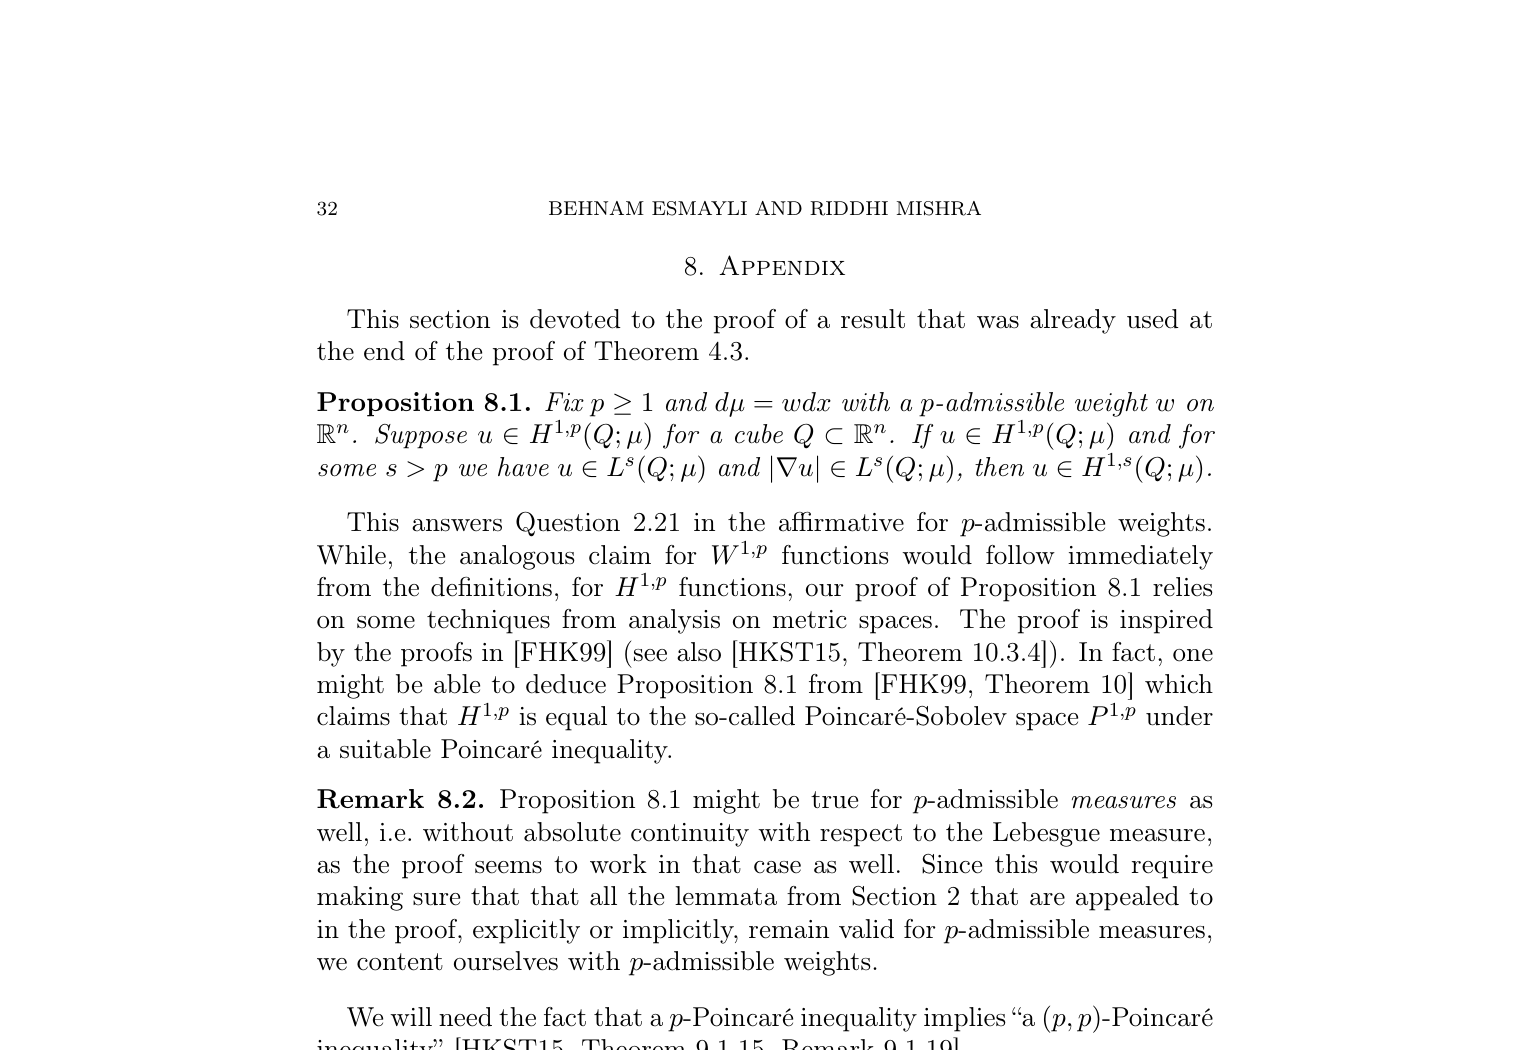
\includegraphics[width=0.98\textwidth]{figures/measure_variant_crop.png}
\end{center}

Here \(\mu\) is \(p\)-admissible in the terminology of \cite{EM}: it is a
Borel doubling measure on \(\R^n\), positive and finite on every cube, and
there is \(C_P\) such that
\begin{equation}\label{eq:PI}
 \avgint_A |f-f_A|\,d\mu
 \le C_P\diam(A)\left(\avgint_A|\nabla f|^p\,d\mu\right)^{1/p}
\end{equation}
for every cube \(A\) and every bounded smooth \(f\) on \(A\).  As recorded
in Section 2.5 of \cite{EM}, doubling and this Poincar\'e inequality give
uniqueness of the Sobolev gradient.  We use that established part of their
framework.

\section{Proof intuition}

The useful part of the source proof is its discrete smoothing.  On a mesh of
size \(h\), replace \(u\) by a smooth partition-of-unity interpolation of its
\(\mu\)-averages over the mesh cubes.  Differences of neighboring averages
are controlled by the original \(p\)-Poincar\'e inequality.  Since
\(\nabla u\in L^s\), H\"older's inequality turns this into a uniform
\(L^s\) bound for the gradients of the smoothings.

The remaining issue is convergence of the functions in \(L^s\).  Applying an
\(s\)-Poincar\'e inequality to \(u\) here would assume the regularity one is
trying to prove.  Instead, doubling supplies the ordinary differentiation
theorem and the \(L^s\)-bounded Hardy--Littlewood maximal operator.  The mesh
averages converge to \(u\) at almost every point and are dominated by
\(C M_\mu u\), so they converge strongly in \(L^s\).  Reflexivity and
Mazur's lemma then close the smooth graph.  None of these steps refers to a
Radon--Nikodym density, Lebesgue convolution, or a distributional derivative.

\section{The result}

\begin{theorem}[measure-valued exponent upgrade]\label{thm:main}
Let \(\mu\) be a \(p\)-admissible Borel measure on \(\R^n\) in the sense
above, let \(1\le p<s<\infty\), and let \(\Omega\subset\R^n\) be open.
Suppose that \(u\in H^{1,p}(\Omega;\mu)\) and that its Sobolev pair satisfies
\[
        u\in L^s(\Omega;\mu),\qquad
        |\nabla u|\in L^s(\Omega;\mu).
\]
Then \(u\in H^{1,s}(\Omega;\mu)\).  Its \(s\)-Sobolev gradient is the same
\(\mu\)-almost everywhere as its \(p\)-Sobolev gradient.
\end{theorem}

Thus Proposition 8.1 of \cite{EM} remains true for arbitrary
\(p\)-admissible measures, as proposed in Remark 8.2.

\section{Preparatory estimates}

We first isolate the only consequence of the Poincar\'e inequality used in
the construction.

\begin{lemma}[nearby averages]\label{lem:averages}
Let \(A,B\) be cubes with \(A\subset B\Subset\Omega\),
\(\ell(B)\le L\ell(A)\), and let \(u\in H^{1,p}(\Omega;\mu)\).  Then
\begin{equation}\label{eq:avgdiff}
 |u_A-u_B|
 \le C_L\diam(B)
       \left(\avgint_B|\nabla u|^p\,d\mu\right)^{1/p}.
\end{equation}
The same estimate, up to twice the constant, controls \(|u_{A_1}-u_{A_2}|\)
when two comparable cubes \(A_1,A_2\) lie in such a cube \(B\).
\end{lemma}

\begin{proof}
Doubling gives \(\mu(B)/\mu(A)\le C_L\).  Hence
\[
 |u_A-u_B|
 \le \avgint_A|u-u_B|\,d\mu
 \le \frac{\mu(B)}{\mu(A)}\avgint_B|u-u_B|\,d\mu,
\]
and \eqref{eq:avgdiff} follows from \eqref{eq:PI}.  For an
\(H^{1,p}\) function, take smooth approximants in the graph norm and pass to
the limit.  This is legitimate because \(\mu(B)<\infty\), so \(L^p(B)\)
convergence implies \(L^1(B)\) convergence.  The two-cube statement follows
by inserting \(u_B\).
\end{proof}

We write \(M_\mu\) for the uncentered Hardy--Littlewood maximal operator over
cubes.  On a doubling metric measure space, \(M_\mu\) is bounded on
\(L^r(\mu)\) for every \(r>1\), and locally integrable functions have
\(\mu\)-almost every point as a differentiation point \cite{Heinonen}.

\begin{lemma}[discrete smoothing on nested cubes]\label{lem:local}
Let \(Q\Subset Q'\Subset\Omega\) be cubes.  Suppose
\(u\in H^{1,p}(Q';\mu)\) and \(u,|\nabla u|\in L^s(Q';\mu)\).  Then
\(u\in H^{1,s}(Q;\mu)\), and the two Sobolev gradients agree on \(Q\).
\end{lemma}

\begin{proof}
For small \(h>0\), take the Euclidean grid \(\{Q_{h,k}\}\) of side length
\(h\) and retain the finitely many cells lying within a fixed multiple of
\(h\) of \(Q\).  They and their fixed dilates lie in \(Q'\).  A standard
smooth partition construction gives nonnegative
\(\varphi_{h,k}\in C^\infty(Q)\) such that
\begin{equation}\label{eq:partition}
 \sum_k\varphi_{h,k}=1,\qquad
 \operatorname{supp}\varphi_{h,k}\subset 3Q_{h,k},\qquad
 |\nabla\varphi_{h,k}|\le C h^{-1},
\end{equation}
with overlap bounded only in terms of \(n\).  Set
\[
       u_h(x)=\sum_k u_{Q_{h,k}}\varphi_{h,k}(x),\qquad x\in Q.
\]
This is smooth.  It has finite \(H^{1,s}\) norm by the estimates below, so it
is an admissible element in the defining smooth class.

Partition \(Q\) measurably among the grid cells.  If \(x\) is assigned to
\(Q_{h,i}\), every index active at \(x\) is a bounded number of cells away.
There is a cube \(R_{h,i}\subset Q'\), of side at most \(C h\), containing
\(Q_{h,i}\) and all active \(Q_{h,k}\); the family
\(\{R_{h,i}\}_i\) has bounded overlap.  From
\(\sum_k\nabla\varphi_{h,k}=0\), Lemma \ref{lem:averages}, and then
H\"older's inequality,
\begin{align}
 |\nabla u_h(x)|
 &=\left|\sum_k(u_{Q_{h,k}}-u_{Q_{h,i}})
                     \nabla\varphi_{h,k}(x)\right| \notag\\
 &\le C\left(\avgint_{R_{h,i}}|\nabla u|^p\,d\mu\right)^{1/p}
 \le C\left(\avgint_{R_{h,i}}|\nabla u|^s\,d\mu\right)^{1/s}.
 \label{eq:pointgrad}
\end{align}
This identity is valid at every point; in particular, no assumption that
grid boundaries are \(\mu\)-null is hidden here.  Raising to the \(s\)-th
power, integrating over the part assigned to \(Q_{h,i}\), and summing gives
\begin{equation}\label{eq:gradbound}
       \|\nabla u_h\|_{L^s(Q;\mu)}
       \le C\|\nabla u\|_{L^s(Q';\mu)}.
\end{equation}
Indeed, the assigned set lies in \(R_{h,i}\), and the enlarged cubes have
bounded overlap.

It remains to prove strong convergence of the function components without
assuming that \(u\) already has \(s\)-Sobolev regularity.  If \(x\) is a
differentiation point of \(u\), every active \(Q_{h,k}\) lies in a cube
centered at \(x\) of side \(C h\).  Doubling compares the measures of these
two comparable cubes.  Consequently
\[
 |u_{Q_{h,k}}-u(x)|
 \le C\avgint_{B_\infty(x,Ch)}|u(y)-u(x)|\,d\mu(y)\longrightarrow0.
\]
Thus \(u_h(x)\to u(x)\) for \(\mu\)-almost every \(x\in Q\).  The same
comparison gives
\begin{equation}\label{eq:maxdom}
       |u_h(x)|\le C M_\mu(u\mathbf1_{Q'})(x).
\end{equation}
Here \(s>p\ge1\), hence \(s>1\).  The doubling maximal theorem makes the
right side an \(L^s\) function.  Dominated convergence now yields
\begin{equation}\label{eq:functionconv}
             u_h\longrightarrow u\quad\hbox{strongly in }L^s(Q;\mu).
\end{equation}

For completeness, realize \(H^{1,s}(Q;\mu)\) as the closure in
\(L^s(Q;\mu)\times L^s(Q;\mu)^n\) of the smooth graph
\(\{(f,\nabla f)\}\).  Since \(s>1\), this closed subspace is reflexive.
Equations \eqref{eq:gradbound} and \eqref{eq:functionconv} show that
\((u_h,\nabla u_h)\) is bounded, with function component converging strongly
to \(u\).  Pass to a weakly convergent subsequence in the closed graph and
apply Mazur's lemma to tail convex combinations.  We obtain smooth functions
\(v_j\) and some \(G\in L^s(Q;\mu)^n\) such that
\[
          (v_j,\nabla v_j)\longrightarrow(u,G)
          \quad\hbox{in }L^s\times L^s{}^n.
\]
Therefore \(u\in H^{1,s}(Q;\mu)\).  Since \(\mu(Q)<\infty\), the same
convergence holds in the \(p\)-graph norm.  Uniqueness of the
\(H^{1,p}\) gradient gives \(G=\nabla u\) almost everywhere.
\end{proof}

We finally record the elementary sheaf-to-global fact in a form that makes
clear that absolute continuity is irrelevant.

\begin{lemma}[local graph closure is global]\label{lem:global}
Let \(1\le r<\infty\).  Suppose a pair \((u,G)\) belongs locally to the
smooth \(H^{1,r}\) graph on \(\Omega\), and
\(u\in L^r(\Omega;\mu)\), \(G\in L^r(\Omega;\mu)^n\).  Then
\((u,G)\in H^{1,r}(\Omega;\mu)\).
\end{lemma}

\begin{proof}
Choose a countable locally finite cover \(\{U_j\}\) with
\(U_j\Subset\Omega\), and a smooth partition of unity \(\{\psi_j\}\)
with \(\operatorname{supp}\psi_j\Subset U_j\).  Let \(\varepsilon_m\downarrow0\).
Local graph membership lets us choose \(f_{m,j}\in C^\infty(U_j)\) so that
\[
 \|f_{m,j}-u\|_{L^r(U_j)}+
 \|\nabla f_{m,j}-G\|_{L^r(U_j)}
 \le \frac{\varepsilon_m2^{-j}}
  {1+\|\psi_j\|_\infty+\|\nabla\psi_j\|_\infty}.
\]
The locally finite sum \(F_m=\sum_j\psi_j f_{m,j}\), with each product
extended by zero off \(U_j\), is smooth on \(\Omega\).  Since
\(\sum_j\psi_j=1\) and \(\sum_j\nabla\psi_j=0\), Minkowski's inequality
gives
\begin{align*}
 \|F_m-u\|_{L^r}
 &\le\sum_j\|\psi_j(f_{m,j}-u)\|_{L^r},\\
 \|\nabla F_m-G\|_{L^r}
 &\le\sum_j\bigl(\|\psi_j(\nabla f_{m,j}-G)\|_{L^r}
       +\|\nabla\psi_j(f_{m,j}-u)\|_{L^r}\bigr)
 \le C\varepsilon_m.
\end{align*}
Thus \((F_m,\nabla F_m)\to(u,G)\) in the global graph norm.  The assumed
global integrability also shows that every \(F_m\) has finite graph norm.
\end{proof}

\section{Proof of Theorem \ref{thm:main}}

Let \(V\Subset\Omega\).  Cover \(\overline V\) by finitely many cubes
\(Q_j\) for which there are enlarged cubes \(Q'_j\Subset\Omega\).
Restriction of a smooth approximating sequence shows
\(u\in H^{1,p}(Q'_j;\mu)\).  Lemma \ref{lem:local} gives
\(u\in H^{1,s}(Q_j;\mu)\), with gradient equal to the original
\(p\)-gradient.  A finite smooth partition of unity therefore shows that the
pair \((u,\nabla u)\) belongs locally to the \(H^{1,s}\) graph throughout
\(\Omega\).  Its two components are globally in \(L^s\) by hypothesis, so
Lemma \ref{lem:global} yields \(u\in H^{1,s}(\Omega;\mu)\), with the asserted
gradient. \qed

\section{Verification, limitations, and novelty}

The proof was audited at the four points where singular measures could matter:
\begin{enumerate}[leftmargin=*]
\item Lemma \ref{lem:averages} is obtained by graph-norm completion and uses
only finite cube measure, doubling, and \eqref{eq:PI}.
\item Equation \eqref{eq:pointgrad} is an algebraic identity for the smooth
partition, so positive measure on grid boundaries causes no loss.
\item Equations \eqref{eq:maxdom}--\eqref{eq:functionconv} are standard
doubling-measure facts and use \(s>1\), including when \(p=1\).
\item Lemma \ref{lem:global} explicitly controls the derivative of the
partition of unity and does not use a Lebesgue density.
\end{enumerate}

This theorem does not address Open Problem A.18 cited in \cite{EM}, which asks
whether every \(p\)-admissible measure on \(\R^n\), \(n\ge2\), is absolutely
continuous.  Instead, it shows that the exponent upgrade remains valid even
without knowing the answer to that problem.

A bounded novelty search was performed through 11 August 2026.  The run
indexes were searched for arXiv:2505.20555 and the exact exponent-upgrade
wording.  Exact web/arXiv searches used the wording of Remark 8.2 and
combinations of ``\(p\)-admissible measure'', ``\(H^{1,p}\)'',
``\(H^{1,s}\)'', and ``discrete convolution''.  The final journal version,
published 10 December 2025, still contains Remark 8.2.  No later resolution or
equivalent maximal-function proof was found.  Novelty confidence is moderate
pending a specialist citation search.

The recommended human-review focus is the off-center differentiation argument
in Lemma \ref{lem:local} and the applicability of the source's gradient-
uniqueness theorem to its exact smooth-test definition of admissibility.

\begin{thebibliography}{9}

\bibitem{EM}
B. Esmayli and R. Mishra,
\emph{On removable sets for weighted Sobolev functions},
Potential Analysis \textbf{64} (2026), article 18;
arXiv:2505.20555v2.
\href{https://doi.org/10.1007/s11118-025-10270-9}
{doi:10.1007/s11118-025-10270-9}.

\bibitem{Heinonen}
J. Heinonen,
\emph{Lectures on Analysis on Metric Spaces},
Universitext, Springer, New York, 2001.

\end{thebibliography}

\end{document}
